\documentclass{article}
\usepackage{polski} % poprawne wyświetlanie polskich znaków
\usepackage[utf8]{inputenc}
\usepackage{color}
\usepackage{graphicx}% paczka do wyświetlenia obrazów, obrazy beda znajdowały się w katalogu głownym wiec nie potrzeby, aby podawać ścieżkę
\usepackage{natbib} % sekcja źródeł
\usepackage{booktabs} % For \toprule, \midrule and \bottomrule
\usepackage{siunitx} % Formats the units and values
\usepackage{pgfplotstable} % Generates table from .csv
\begin{document}
\begin{figure}
    \centering
    
\includegraphics[scale=0.15]{wsb-s}
\end{figure}
\title{\color{blue}Projektowanie Zaawansowane \\ - projekt zaliczeniowy}
\author{Michał Kotowski \\ Bartosz Górny \\ Dawid Bieńkowski \\ Bartek Turkosz}
\date{Czerwiec 2020}
\maketitle

\section{Założenia projektowe}
\subsection{Problem badawczy}
\qquad Oszacowanie ilości wypadków drogowych w Polsce w latach 2019 - 20XX na podstawie danych z lat 2000-2018 przy wykorzystaniu matematycznych modeli rozwiązywania zadań.

\subsection{Teoria opracowania}
\qquad Po przeanalizowaniu założonego celu oraz pobranych danych doszliśmy do wniosku, iż  realizowane zadanie ma charakter czysto regresyjny. Wybraliśmy odpowiednio dwie metody: regresja liniowa metodą najmniejszych kwadratów błędów i regresja wielomianowa wykorzystując aproksymację wielomianową średnio kwadratową.
\begin{itemize}
    \item Regresja liniowa:
    rozwiązanie zadania przedstawioną metodą polega na wyznaczeniu linii trendu w postaci $y=ax+b$, gdzie a i b to współczynniki, których poszukujemy realizując minimalizacje podanej sumy:
    \begin{center}
       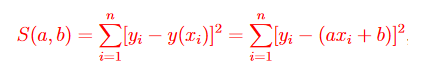
\includegraphics{sumareglin} 
    \end{center}
Należy zaznaczyć, że różnice miedzy dokładnymi ${y_i}$ oraz wartościami obliczonymi z równania prostej są podniesione do kwadratu, aby uniknąć możliwości, że będą się nawzajem znosiły na skutek różnicy znaków
    \item Regresja wielomianowa: jest to sposób obliczenia zależności między zmienną zależną a jedną lub więcej zmiennymi niezależnymi występującymi w wyższych potęgach. W przypadku jednej zmiennej niezależnej równianie regresji przyjmuję postać:
    \begin{center}
       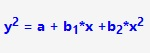
\includegraphics{regwiel1.jpg} 
    \end{center}
    Wykorzystując aproksymację średnio kwadratową, wykorzystując wzór:
    \begin{center}
       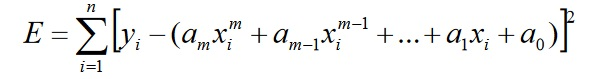
\includegraphics[scale=0.5]{regwiel2.jpg} 
    \end{center}
    należy wyznaczyć $a_i$ funkcji E takich że pochodne cząstkowe względem $a_i$ są równe 0. Poniżej przedstawiamy rozpisany proces wyznaczania $a_i$ dla wielomianu kwadratowego.
    \begin{center}
        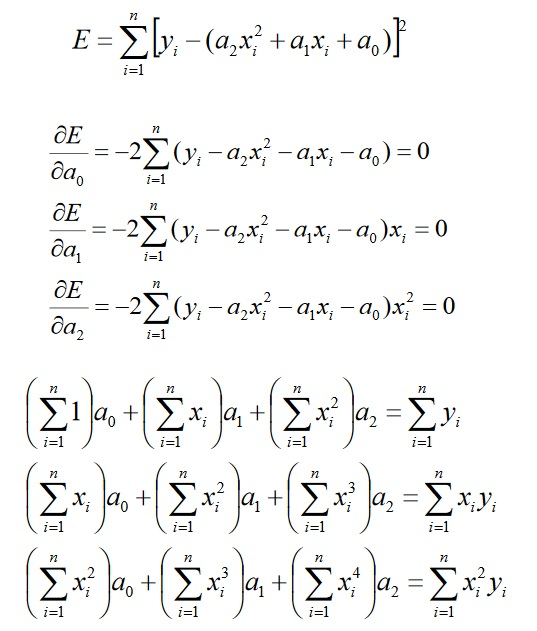
\includegraphics[scale=0.5]{regwiel3.jpg}\newline
    \end{center}
    \end{itemize}
\subsection{Przedstawienie danych}
\qquad Dane zostały pobrane w formacie .csv ze strony Głównego urzędu statystycznego: \textit{https://stat.gov.pl/} zatem przedstawiają one realne wartości dla analizowanego problemu. Poniżej zestawienie tabelaryczne.
% Setup siunitx:
\sisetup{
  round-mode          = places, % Rounds numbers
  round-precision     = 1, 
}

\begin{table}[h!]
  \begin{center}
    \caption{Dane z GUS na temat ilości wypadków w Polsce w latach 2000-2018.}
    \label{table1}
    \pgfplotstabletypeset[
      multicolumn names, % allows to have multicolumn names
      col sep=comma, % the seperator in our .csv file
      display columns/0/.style={
		column name=$Lp.$, % name of first column
		column type={S},string type},  % use siunitx for formatting
      display columns/1/.style={
		column name=$Rok$,
		column type={S},string type},
	display columns/2/.style={
		column name=$Dane$,
		column type={S},string type},
    display columns/3/.style={
		column name=$Sumarycznie$,
		column type={S},string type},
      every head row/.style={
		before row={\toprule}, % have a rule at top
		after row={\midrule} % rule under units
			},
		every last row/.style={after row=\bottomrule}, % rule at bottom
    ]{dane.csv} % filename/path to file
  \end{center}
\end{table}
\section{Przedstawienie wyników}
\subsection{Regresja liniowa - zrealizowana na podstawie kodu źródłowego na przeprowadzonych zajęciach}
 \begin{center}
        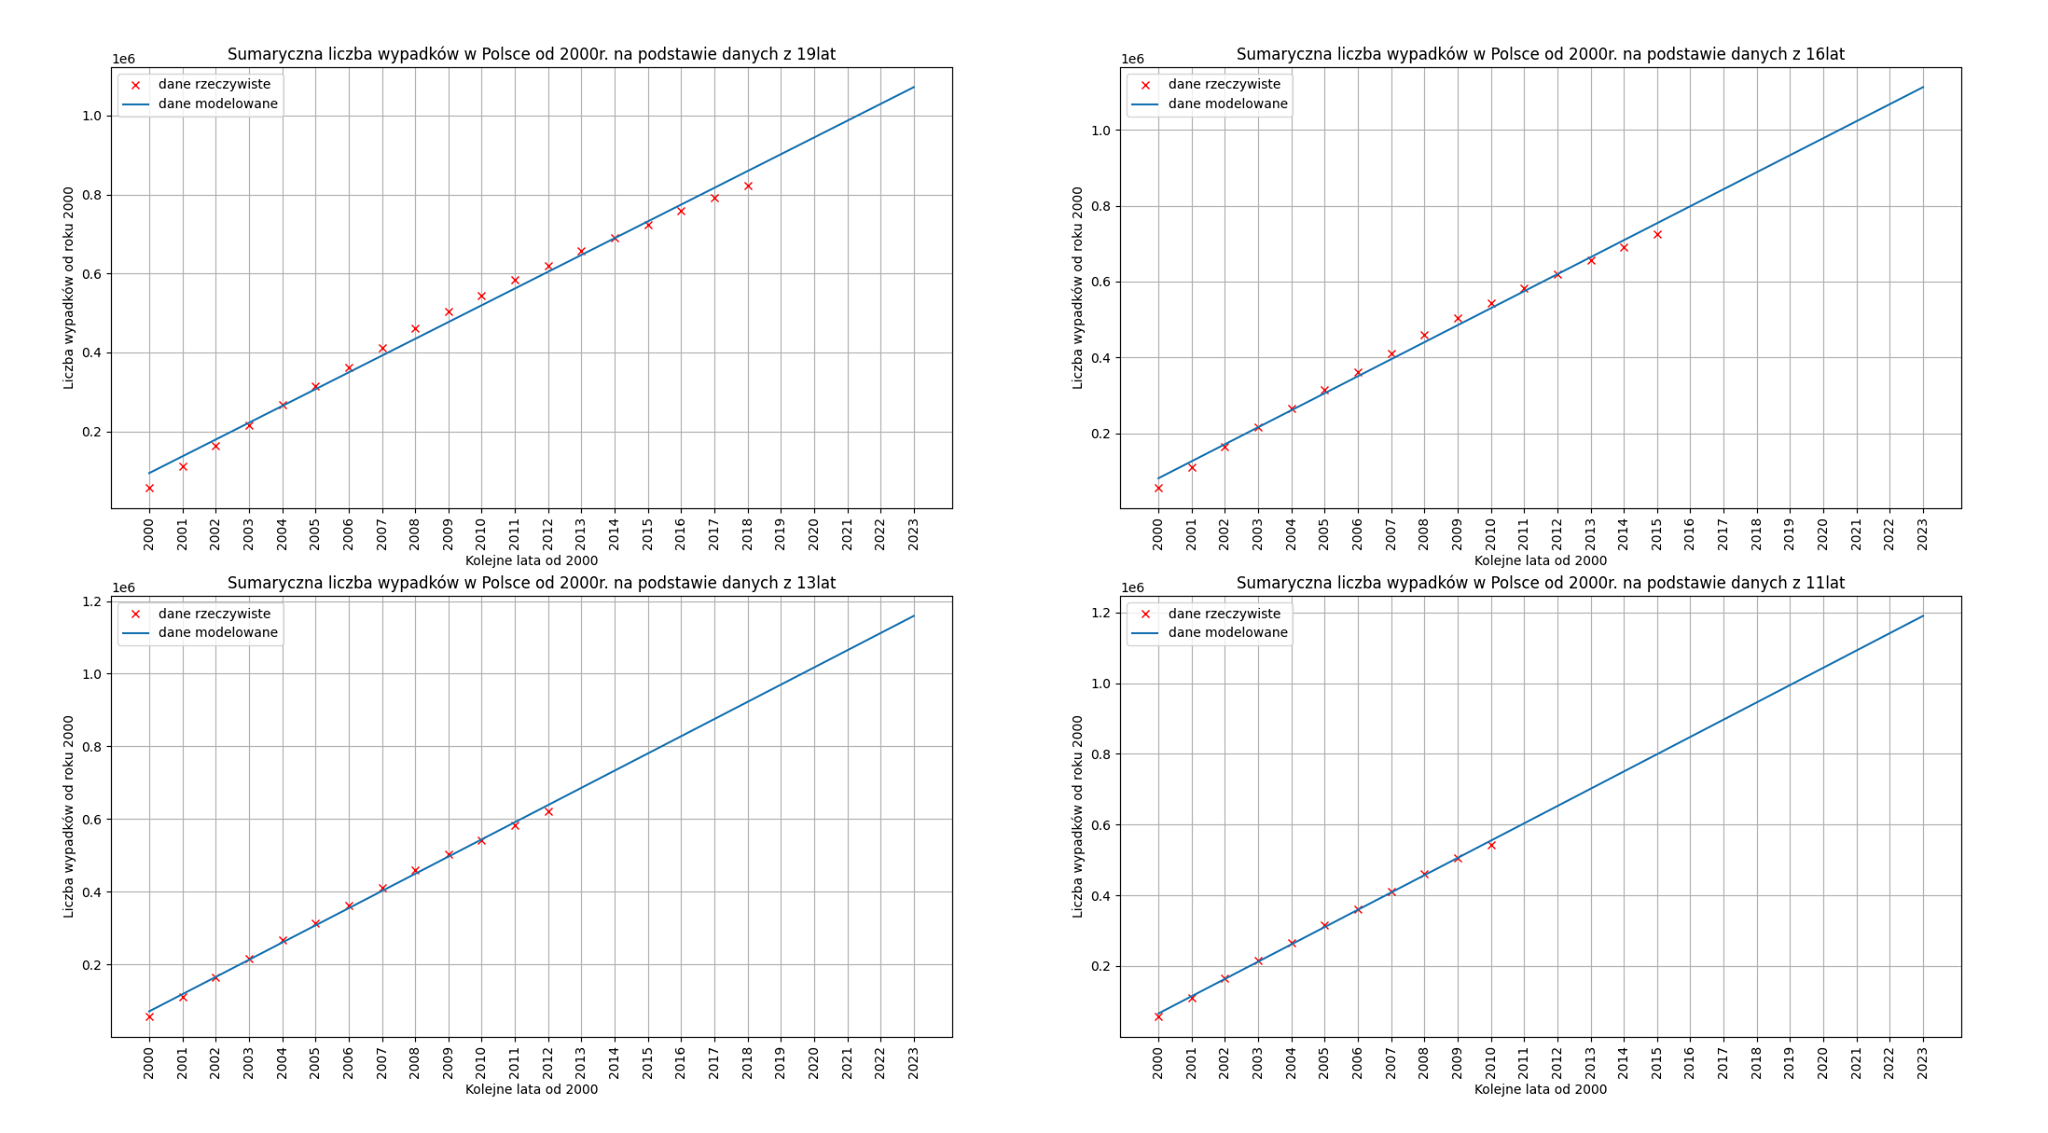
\includegraphics[scale=0.18]{liniowareczny.jpg}
    \end{center}
\subsection{Regresja liniowa - zrealizowana przy wykorzystaniu biblioteki sklearn}
 \begin{center}
        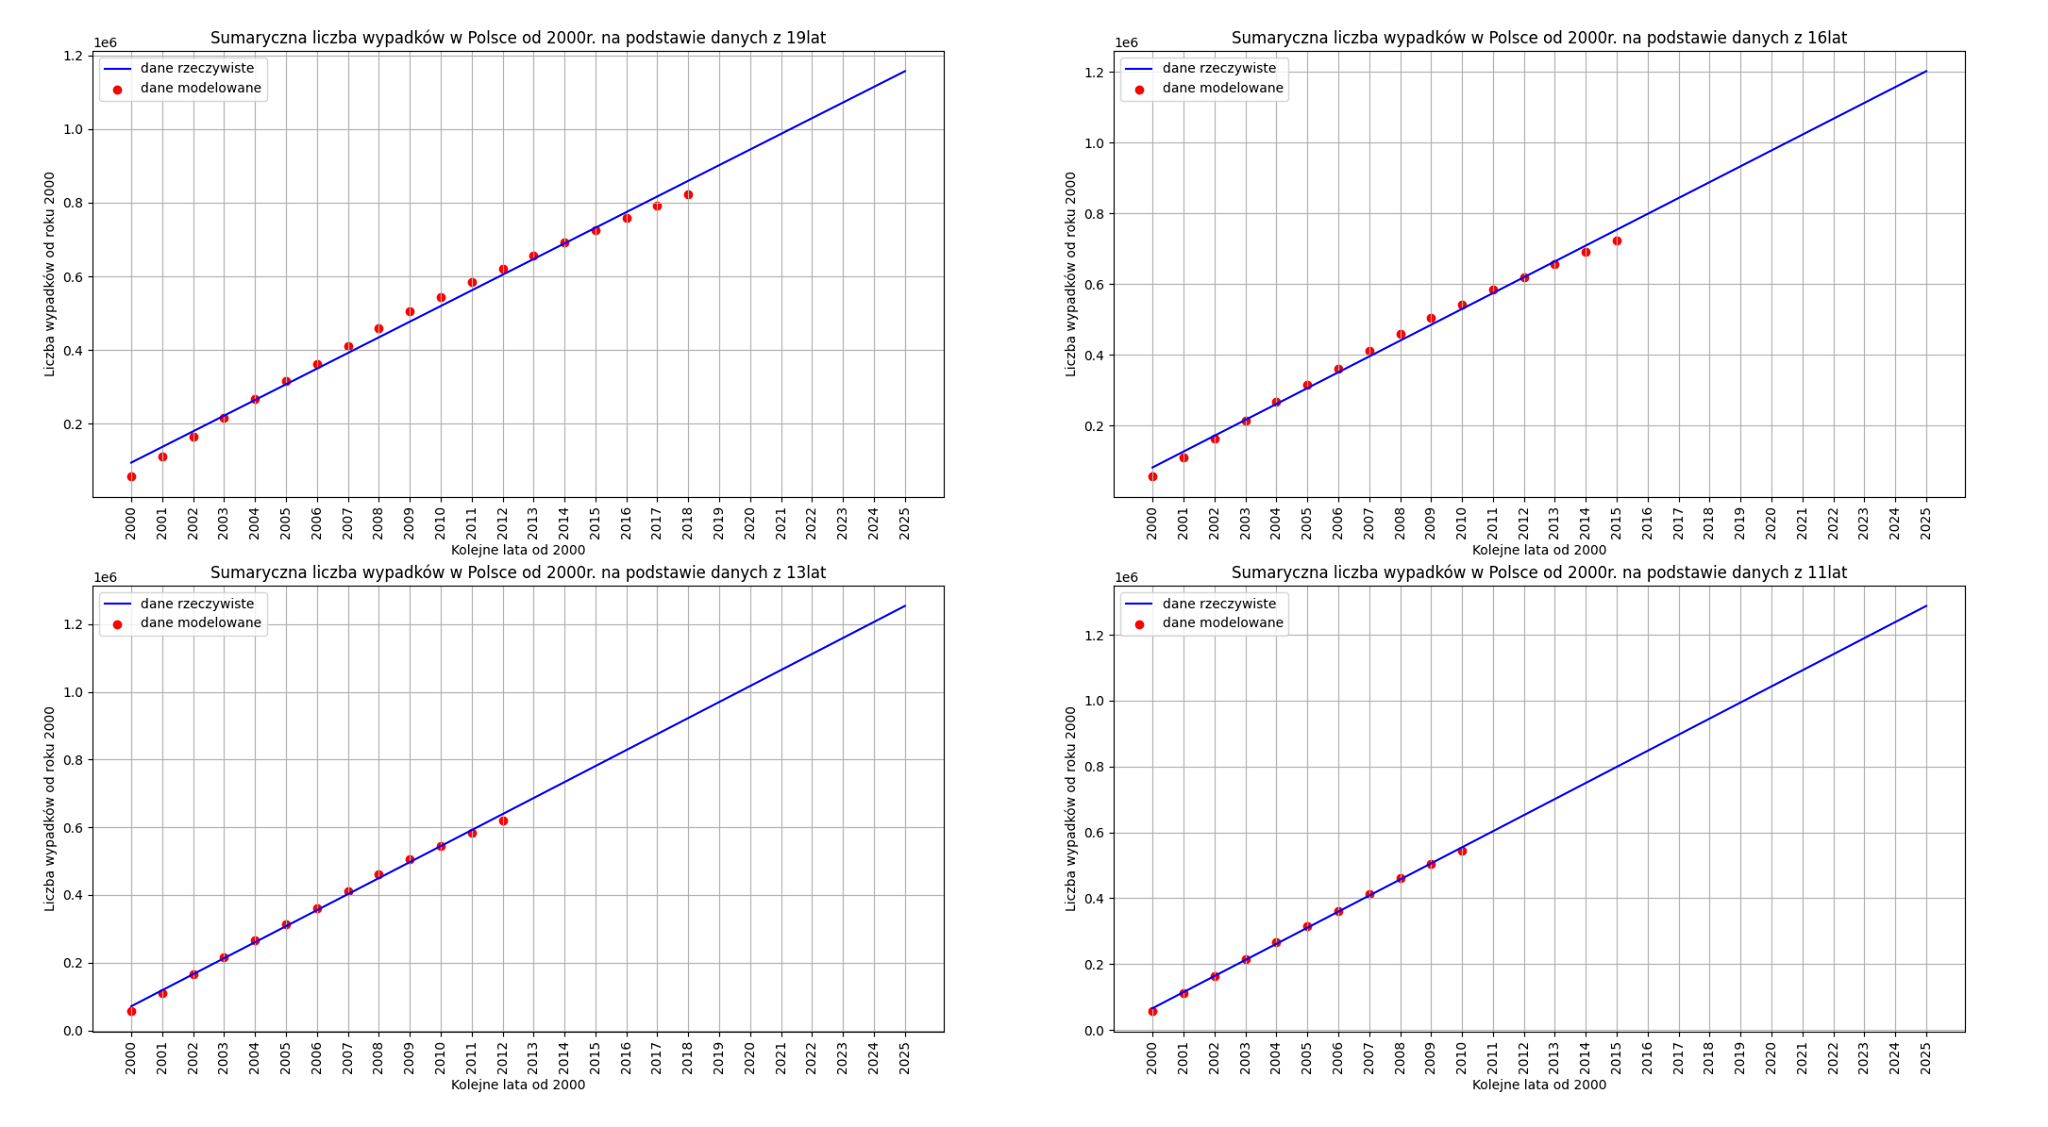
\includegraphics[scale=0.18]{liniowabiblioteka.jpg}
    \end{center}
\subsection{Regresja wielomianowa - zrealizowana na podstawie kodu źródłowego na przeprowadzonych zajęciach}
 \begin{center}
        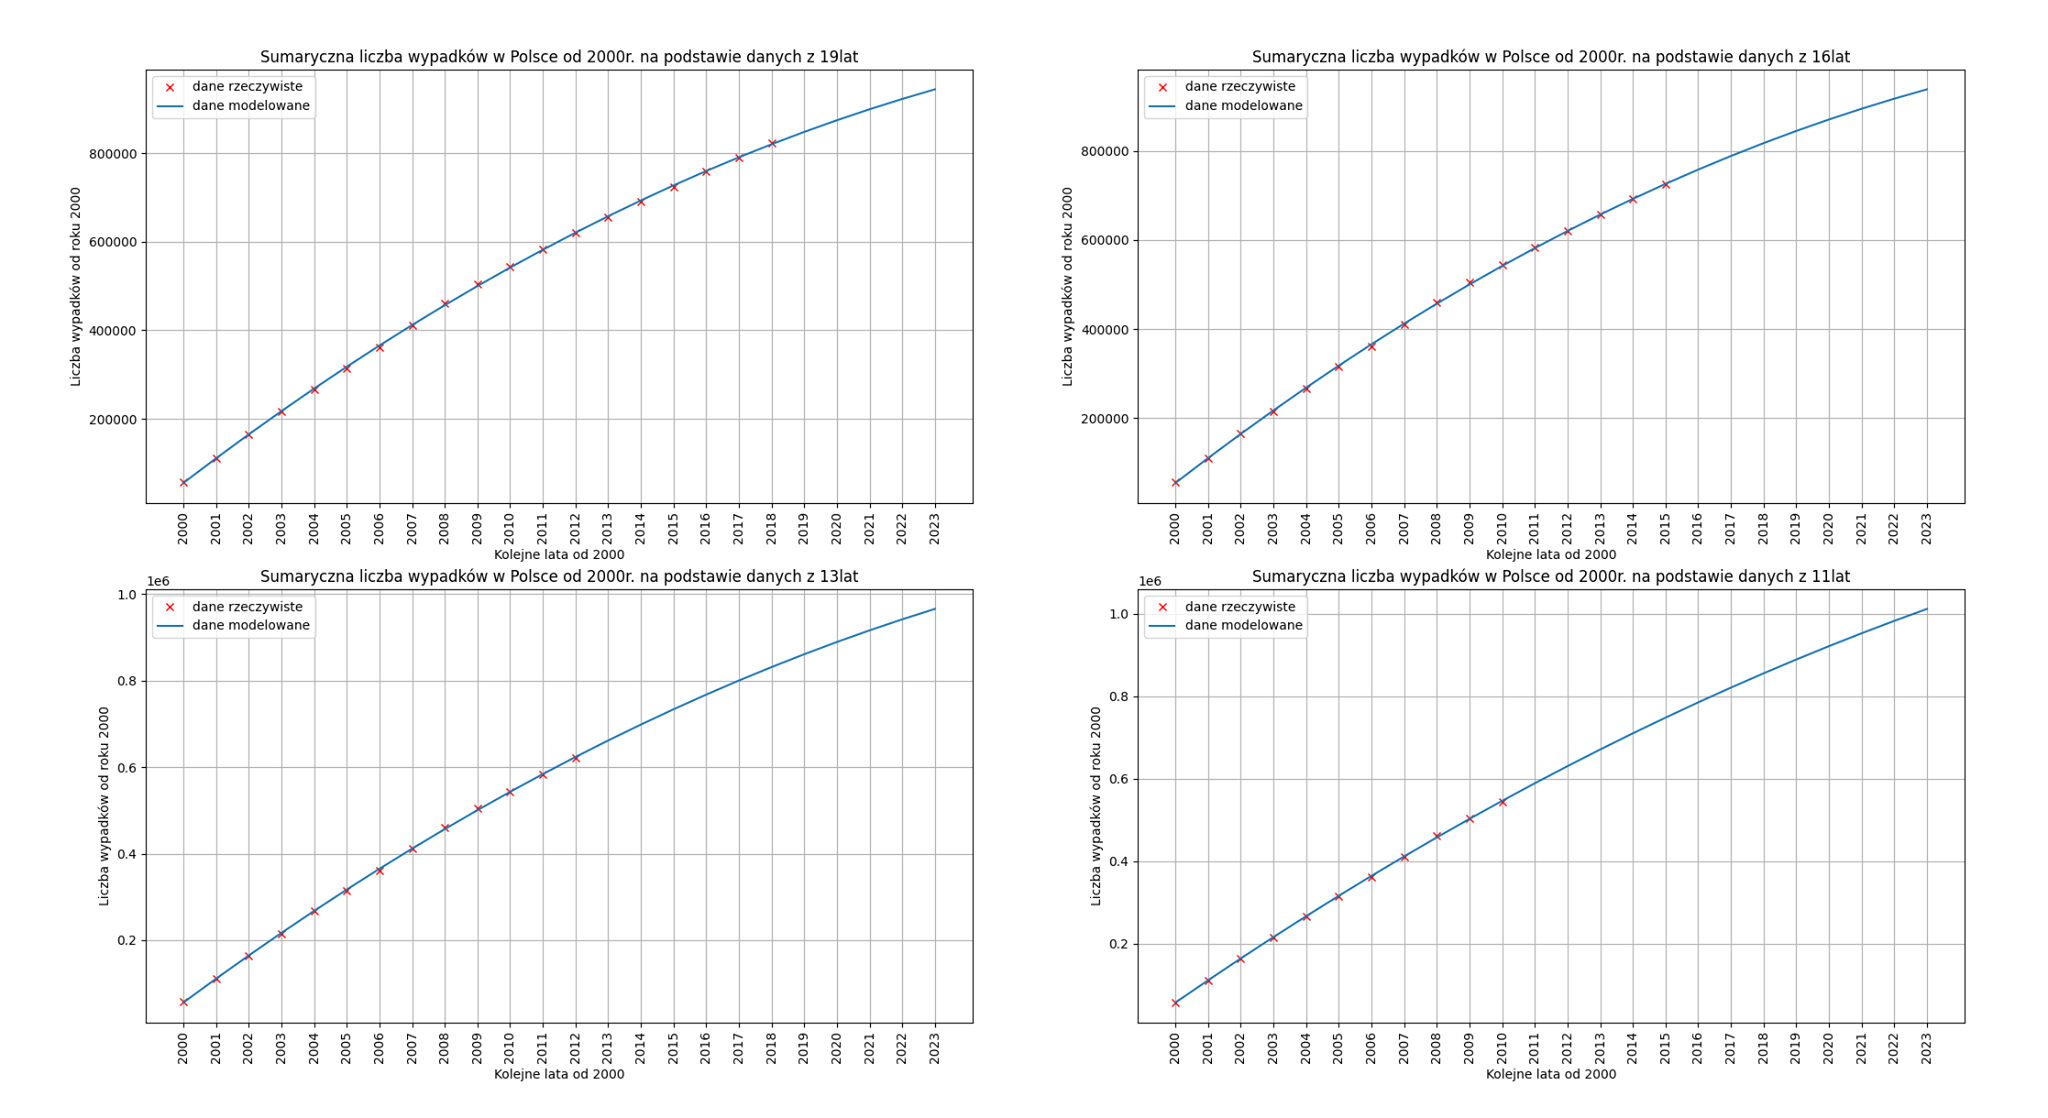
\includegraphics[scale=0.18]{wielomianreczny.jpg}
    \end{center}
\subsection{Regresja wielomianowa - (kwadratowa) zrealizowana przy wykorzystaniu biblioteki sklearn}
 \begin{center}
        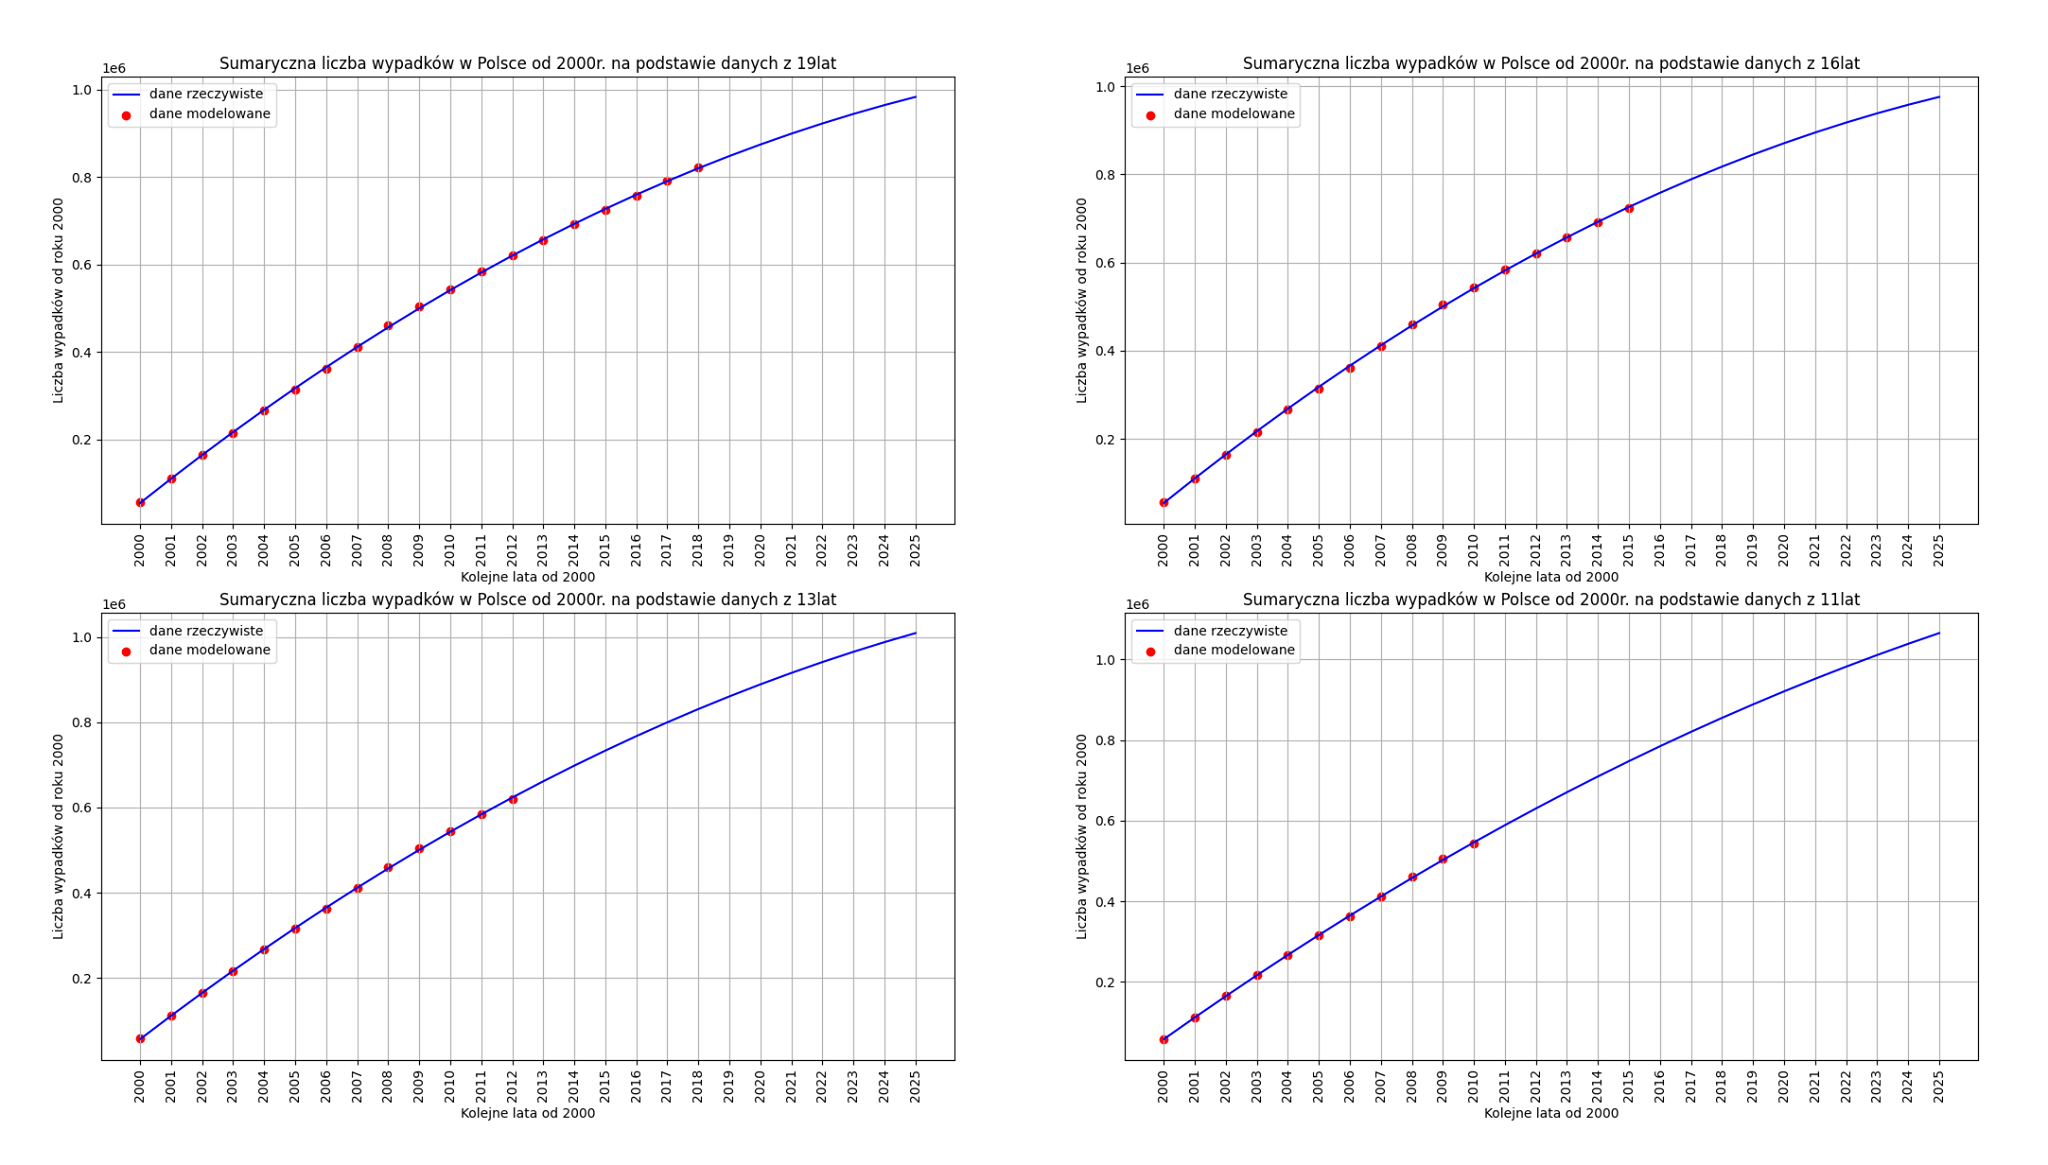
\includegraphics[scale=0.18]{wielomianbiblioteka.jpg}
    \end{center}
\section{Wnioski}
\qquad Ze względu na charakter badanej wartości oraz niewielką ilość zmiennych, po przeprowadzonej analizie można wywnioskować iż modelem przedstawiającym wyniki najbardziej zbliżone to rzeczywistych jest model regresji wielomianu kwadratowego, zarówno ten realizowany za pomocą biblioteki sklearn jak również algorytm pisany ręcznie (obie funkcje nieznacznie się różnią) . W dalszych latach można zaobserwować spłaszczenie wykresu, wartości nie rosną już tak gwałtownie. To oznacza ze model regresji liniowej, im dalej w przyszłość tym z większą niedokładnością szacowane są dane, natomiast wielomian kwadratowy pozwala nam na zniwelowanie poziomy błędu. Ponadto należy stwierdzić, że wprowadzenie dodatkowych zmiennych niezależnych takich jak np. opady roczne, ilość pojazdów ogółem czy średnia temperatura pozwoliła by na doprecyzowanie modelu.
\section{Podział zadań}
Proces decyzyjny dotyczący realizowanego problemu projektowego realizowaliśmy poprzez tzw. burzę mózgów przez komunikator, następnie podzieliliśmy się pracą na dwa mniejsze zespoły.
\begin{itemize}
    \item Michał Kotowski:
    analiza problemu i zebranie danych, regresja wielomianowa kod, przygotowanie dokumentacji
    \item Bartosz Górny:
    analiza problemu i zebranie danych, regresja wielomianowa kod, przygotowanie dokumentacji
    \item Dawid Bieńkowski:
    analiza problemu i zebranie danych, regresja liniowa kod
    \item Bartek Turkosz:
    analiza problemu i zebranie danych, regresja liniowa kod
\end{itemize}
\section{Źródła:}
\textit{$http://www.math.uni.wroc.pl/~dpilarcz/dydaktyka/bio12/W_4.pdf$}\\
\textit{$http://www.if.pw.edu.pl/~agatka/numeryczne/wyklad_05.pdf$}\\
\textit{$https://bdl.stat.gov.pl/BDL/metadane/cechy/2423$}\\
\textit{$https://www.latex-tutorial.com/tutorials/pgfplotstable/$}\\
\textit{$https://scikit-learn.org/stable/$}\\
\end{document}
s